\let\negmedspace\undefined
\let\negthickspace\undefined
\documentclass[journal]{IEEEtran}
\usepackage[a5paper, margin=10mm, onecolumn]{geometry}
\usepackage{tfrupee}  % Include tfrupee package
\usepackage{gvv-book}
\usepackage{gvv}
\usepackage{cite}
\usepackage{amsmath, amssymb, amsfonts, amsthm}
\usepackage{algorithmic}
\usepackage{graphicx}
\usepackage{textcomp}
\usepackage{xcolor}
\usepackage{txfonts}
\usepackage{listings}
\usepackage{enumitem}
\usepackage{mathtools}
\usepackage{gensymb}
\usepackage{comment}
\usepackage[breaklinks=true]{hyperref}
\usepackage{tkz-euclide}
\usepackage{longtable}
\usepackage{multirow}
\usepackage{hhline}
\usepackage{lscape}
\usepackage{inputenc}  % Automatically handles various encodings

\setlength{\headheight}{1cm}  % Set header height
\setlength{\headsep}{0mm}     % Set header separation
\setlength{\intextsep}{10pt}  % Space between text and floats

\numberwithin{equation}{enumi}
\numberwithin{figure}{enumi}
\renewcommand{\thetable}{\theenumi}

\begin{document}

\bibliographystyle{IEEEtran}
\vspace{3cm}

\title{9.2.9}
\author{EE24BTECH11020 - Ellanti Rohith}
\maketitle

\renewcommand{\thefigure}{\theenumi}
\renewcommand{\thetable}{\theenumi}

\textbf{Question}: Find the solution of the differential equation $
y^{2}y' + y^2 + 1 = 0$ and verify if $ x + y = \tan^{-1}(y) $ is a solution.
\\
\vspace{3.5pt}


\textbf{Theoretical Solution:} \\
Given the differential equation:
\begin{align}
y^{2} \frac{dy}{dx} + y^2 + 1 = 0
\end{align}
Rearranging:
\begin{align}
y^{2} \frac{dy}{dx} = -y^{2} - 1
\end{align}
Dividing both sides by $ y^2 $:
\begin{align}
\frac{dy}{dx} = -1 - \frac{1}{y^2}
\end{align}
This simplifies to:
\begin{align}
\frac{dy}{-1 - \frac{1}{y^2}} = dx
\end{align}
\begin{align}
\frac{-y^2 dy}{y^2 + 1} = dx
\end{align}
Adding and subtracting 1 in the numerator of  LHS:
\begin{align}
\frac{(-y^2 + 1 - 1) dy}{y^2 + 1} = dx
\end{align}
\begin{align}
- dy + \frac{dy}{y^2 + 1} = dx
\end{align}
Integrating both sides:
\begin{align}
\int -dy + \frac{dy}{y^2 + 1} = \int dx
\end{align}
\begin{align}
-y + \tan^{-1}(y) = x + C
\end{align}
Let the initial condition be $ x_0 = 0 $, $ y_0 = 0 $, then $ C = 0 $, and we have:
\begin{align}
x + y = \tan^{-1}(y)
\end{align}
Thus, $ x + y = \tan^{-1}(y) $ is indeed a solution.\\
\textbf{Simulated solution:} \\
The difference equation is given by:
\begin{align}
y_{n+1} = y_{n} + h \frac{dy}{dx}
\end{align}
\begin{align}
y_{n+1} - y_{n} = h \frac{dy}{dx}
\end{align}
Given that:
\begin{align}
\frac{dy}{dx} = -1 - \frac{1}{y^2}
\end{align}
The difference equation becomes:
\begin{align}
y_{n+1} = y_{n} + (-1 - \frac{1}{y^2})h
\end{align}
However, this method provides inaccurate results since $ \frac{dy}{dx} \to \infty $ as $ y \to 0 $. To fix this, we use the finite differences algorithm as follows:\\
The difference equation is:
\begin{align}
y_{n+1} = y_{n} + h
\end{align}
\begin{align}
x_{n+1} = x_{n} + h \frac{dx}{dy}
\end{align}
Given that:
\begin{align}
\frac{dx}{dy} = \frac{-y^2}{1 + y^2}
\end{align}
The difference equation becomes:
\begin{align}
x_{n+1} - x_{n} = \frac{-h y^2_{n}}{1 + y^2_{n}}
\end{align}
Taking  initial point as $x_{0}=0, y_{0}=0$ and iterating difference equation.\\
Verifying Algoritham,\\
    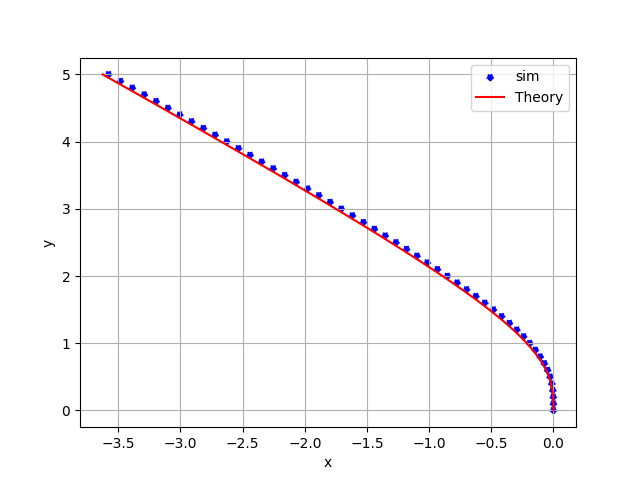
\includegraphics[width=\columnwidth]{Figs/Figure_1.png} 

Thus, We have numerically verified $x+y=\tan^{-1}(y) $ is a solution to given differential equation.

\end{document}
